\documentclass{article}
\usepackage{tikz}
\usepackage{pgfplots}
\usepackage{amssymb}
\usepackage{pgfplotstable}
\usetikzlibrary{shapes}
\usetikzlibrary{arrows,decorations.pathmorphing,backgrounds,positioning,fit,petri}
\usetikzlibrary{arrows.meta,fit,shapes.arrows}
\usepackage{caption} 
\usepackage{xcolor}
\usepackage{subfig}

\definecolor{ured}{RGB}{231,76,60}
\definecolor{ublue}{RGB}{52,152,219}
\definecolor{udark}{RGB}{77,153,77}
\definecolor{orange}{RGB}{255,165,0}

\pgfplotsset{
    width=0.82\textwidth,
    height=0.3\textheight,
    grid=major,
    major grid style={dotted},
    symbolic x coords={1,2,3,4},
    enlarge y limits={upper,value=0.05},
    legend style={
        fill,
        at={(0.5,1.2)},
        anchor=south
    },
}

\tikzset{global scale/.style={
    scale=#1,
    every node/.append style={scale=#1}
}}

\begin{document}

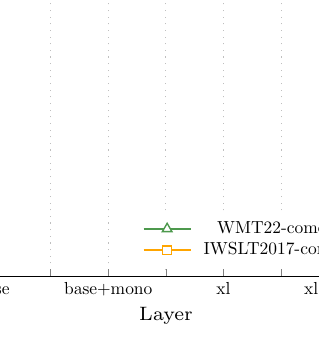
\begin{tikzpicture}
%%%%%%%%%%%%%%%%%%%%%%%%%%%%%%%%%%%%%%%%%%  
\useasboundingbox (13em,-1em) rectangle (3.5em,10em);
%%%%%%%%%%%%%%%%%%%%%%%%%%%%%%%%%%%%%%%%%%%%%%
\begin{axis}[
    global scale = 0.63,
    at={(1em,1em)},
    xtick pos=left,
    axis y line*=left,
    bar width=0.2cm,
    ymin=16, ymax=32,
    ytick={16,18,20,22,24,26,28,30,32},
    xtick={1,2,3,4},
    xticklabels={base,base+mono,xl,xl+mono},
    yticklabels={16,18,20,22,24,26,28,30,32},
    ylabel style={align=center},
    xtick=data,
    xticklabel style={
        inner sep=0pt,
        anchor=north,
        rotate=0,
        yshift=-3pt
    },
    yticklabel style={
        /pgf/number format/fixed,
        /pgf/number format/fixed zerofill,
        /pgf/number format/precision=0,
        rotate=0,
        scaled y ticks=false
    }
]              
    \addplot[sharp plot,ured,smooth,thick,line width=0.5pt,mark=*,mark size=1.4pt,thick,mark options={fill=ured,draw=ured,line width=0.5pt}] 
    plot coordinates {
        (1,17.49244746) (2,20.31124082) (3,21.88275432) (4,24.54456721)
    };\addlegendentry{WMT-BLEU}              

    \addplot[sharp plot,ublue,smooth,thick,line width=0.5pt,mark=pentagon*,mark size=2pt,thick,mark options={fill=white,draw=ublue,line width=0.5pt}] 
    plot coordinates{
        (1,17.49244746) (2,27.18027891) (3,28.35890657) (4,31.04738424)
    };\addlegendentry{IWSLT2017-BLEU}
\end{axis}
\begin{axis}[
    global scale = 0.63,
    at={(1em,1em)},
    legend entries={3,4},
    ymajorgrids=true,
    xmajorgrids=true,
    legend style={
        draw=none,
        line width=1pt,
        at={(15em,1em)},
        column sep=3pt,
        yshift=-5pt,
        anchor=south
    },
    axis y line*=right,
    xticklabels={},
    ymin=70, ymax=84,
    ytick={70,72,74,76,78,80,82,84},
    yticklabels={70,72,74,76,78,80,82,84},
    yticklabel style={
        /pgf/number format/fixed,
        /pgf/number format/fixed zerofill,
        /pgf/number format/precision=0,
        rotate=0
    }
]
    \addplot[sharp plot,udark,smooth,thick,line width=0.5pt,mark=triangle*,mark size=2pt,thick,mark options={fill=white,draw=udark,line width=0.5pt}] 
    plot coordinates {
        (1,71.26040225) (2,74.20203974) (3,77.15428521) (4,80.26201353)
    };\addlegendentry{WMT22-comet22}

    \addplot[sharp plot,orange,smooth,thick,line width=0.5pt,mark=square*,mark size=1.6pt,thick,mark options={fill=white,draw=orange,line width=0.5pt}] 
    plot coordinates {
        (1,76.42141589) (2,78.92049729) (3,80.7341152) (4,83.04977006)
    };\addlegendentry{IWSLT2017-comet22}
\end{axis}
\node at (8.5em,-0.4em){\scriptsize Layer};

\node [rotate=90] at(-1.3em,4.9em){\scriptsize BLEU};
\node [rotate=270] at(18.2em,5em){\scriptsize Comet22};
\end{tikzpicture}

\end{document}